\chapter{Resultados Experimentales}
\label{chap:Resultados}
\lettrine{E}{n} este capitulo expondremos los resultados obtenidos al ejectutar nuesto algoritmo en un entorno de pruebas. Tambien explicaremos este entorno y como se obtuvieron los datasets utilizados para la obtención de las métricas.

\section{Entorno de pruebas}
A continuación explicaremos como se obtuvieron los datasets para realizar donde se realizaron estas pruebas. 
Para la obtencion del dataset se siguio un procedimiento que podemos ver en la figura \ref{fig:flugdataset} ahora explicaremos cada paso

\begin{figure}[h]
\centering
    \includegraphics[width=10cm]{imaxes/mermaid-diagram-2023-09-02-195044.png}
    \caption{Diagrama de flujo para obtención del dataset}
    \label{fig:flugdataset}
\end{figure}

\subsection{Obtencion del tile de un repositorio}
Primero tenemos que buscar un repositorio de datos LiDAR y seleccionar los tiles que usaremos. En nuestro caso obtamos por usar el repositorio de Luxemburgo \cite{luxdata} como ya se comento en el sección \ref{chap:investigPlan}.Se escogió este principalmente por su densidad de puntos que cumple con lo requerido y por ser libre para que cualquiera pueda usarlo.
Para nuestro dataset escogimos los tiles con identificador \textit{57000\_105000} y \textit{81500\_82500}.

\begin{figure}[h]
  \begin{subfigure}{0.5\textwidth}
    \centering
    \includegraphics[scale=0.30]{imaxes/tile1.png}
    \caption{Tile 81500\_82500}
    \label{fig:tile1}
  \end{subfigure}
  \begin{subfigure}{0.5\textwidth}
    \centering
    \includegraphics[scale=0.30]{imaxes/tile2.png}
    \caption{Tile 57000\_105000}
    \label{fig:tile2}
  \end{subfigure}
  \label{fig:restiles}
\end{figure}

\subsection{Preparación del Tile}
Como ya comentamos en el capitulo \ref{chap:Deteccion} necesitamos obtener un tile con las alturas normalizadas y con el ultimo retorno.A partir de eso necesitamos la versión con suelo para el mapa de alturas y otro sin el suelo para la detección. La explicación de como obtenerlos la encontramos en el capitulo \ref{chap:normalAlgo} , \ref{chap:LastAlgo} y \ref{chap:groundAlgo}.

\subsection{Recortar Tile en Tiles mas pequeños}
Para el entorno de prueba se decidió optar por recortar los tiles en trozos mas pequeños.Esto se decidió por que el ground truth se hace manera manual y por lo tanto generarlo para un tile tan grande seria prácticamente imposible y se cometerían muchos errores. Además también eliminas puntos que no son de interés como campos de cultivos o casas que lo único que hacen es ralentizar el proceso de prueba.

Para esta tarea se realizó un pequeño programa para recortar un tile grande en tiles mas pequeños cuadrados y todos del mismo tamaño. Después de esto escogeremos manualmente varios donde veamos que haya arboles y con diferentes tipos. En nuestro caso el dataset esta formado por 70 de estos tiles y con un total de 547 arboles de diferentes especies para que las métricas obtenidas sean reales.

\begin{figure}[h]
\centering
\begin{subfigure}[t]{.5\textwidth}
  \centering
  \includegraphics[height=5cm]{imaxes/subtile1.png}
\end{subfigure}%
\begin{subfigure}[t]{.5\textwidth}
  \centering
  \includegraphics[height=5cm]{imaxes/subtile2.png}
\end{subfigure}

\begin{subfigure}[t]{.5\textwidth}
  \centering
  \includegraphics[height=5cm]{imaxes/subtile3.png}
\end{subfigure}%
\begin{subfigure}[t]{.5\textwidth}
  \centering
  \includegraphics[height=5cm]{imaxes/subtile4.png}
\end{subfigure}

\caption{Ejemplo de tiles recortados}
\label{fig:ejemplotree}
\end{figure}

\subsection{Obtencion del Ground Truth}
Una vez con los tiles preparados necesitamos un ground truth con la ubicación de los arboles.Para esta tarea tambien se desarrollo un pequeño programa para marcar estos mediante una interfaz gráfica como vemos en la figura \ref{fig:labelTile}.
En esta interfaz se nos muestra la nube de puntos y al hacer \textit{Shit} + \textit{Click Izquierdo} marcamos el punto donde esta el árbol, idealmente marcaremos donde se encuentre el tronco, en los casos donde no se pueda saber bien si es el tronco marcaremos la copa del árbol.

Una vez los seleccionemos todos al cerrar la interfaz se nos generara un archivo \textit{csv} con las coordenadas de los puntos. Este archivo es el que usaremos en un futuro para comprobar la precisión de la detección.

\section{Equipo de Pruebas}
Una vez con el dataset obtenido, comentaremos el equipo donde se realizaron estas pruebas. Para los test usamos una PC de sobremesa con las especificaciones que podemos ver en esta tabla 

\begin{table}[h]
\centering
\rowcolors{2}{white}{udcgray!25}
\begin{tabular}{c|c}
\rowcolor{udcpink!25}
\textbf{Especificación} & \textbf{Valor} \\\hline

CPU & Ryzen 5 1600 6c 12t 3.20 GHz\\
Memoria RAM & 16 gb 2666 mhz \\
GPU & Nvidia GTX 1060 6 gb \\
OS & Windows 10 Home 22H2 \\


\end{tabular}
\caption{Tabla con el desglose de los costes humanos}
\label{tabcospes}
\end{table}


\begin{figure}[h]
\centering
    \includegraphics[width=7cm]{imaxes/marking.png}
    \caption{Programa para marcar los arboles}
    \label{fig:labelTile}
\end{figure}

\section{Parámetros de Prueba}

Antes de revisar los resultados de las pruebas, es esencial definir los parámetros utilizados en su realización. En primer lugar, estableceremos la resolución del mapa de alturas, que influye en la calidad y la resolución del mapa. Esta variable se establecerá en \textit{\textbf{0.005}}. A continuación, determinaremos el tamaño de la vecindad, en este caso, \textit{\textbf{80}}, y el umbral necesario para determinar si un valor es un máximo, que se fijará en \textit{\textbf{0.3}}.

En lo que respecta a la detección por estratos, estableceremos el número mínimo de puntos requeridos para considerar que un objeto es un árbol, que será \textit{\textbf{40}}. Además, definiremos el tamaño de los "slices" como \textit{\textbf{1}}, y el umbral necesario para determinar si el ajuste de la línea es suficientemente bueno, que será \textit{\textbf{0.1}}.

A continuación, presentaremos estos valores en una tabla \ref{tablavar} para una visualización más rápida.
\begin{table}[h]
\centering
\rowcolors{2}{white}{udcgray!25}
\begin{tabular}{c|c}
\rowcolor{udcpink!25}
\textbf{Especificación} & \textbf{Valor} \\\hline

Resolución del mapa de altura & 0.005 \\
Tamaño de vecindad & 80 \\
Umbral detección en máximos & 0.3 \\
Mínimo de puntos por estrato & 40 \\
Tamaño de "Slice" & 1 \\
Umbral Linealidad & 0.1 \\


\end{tabular}
\caption{Tabla con el valor de las constantes}
\label{tablavar}
\end{table}

\section{Resultados}
En esta sección comentaremos los resultados obtenidos y las métricas obtenidas tras los test en el conjunto de datos obtenido mediante el proceso anteriormente explicado.

Para poder entender lo que pasa en el sistema necesitamos una manera de cuantificar que tan bien esta funcionando, para esta cuantificación se usaron las métricas mas comunes en el campo de clasificación, la \textit{precisión}, la \textit{especialidad}, la \textit{exactitud} y la \textit{sensibilidad}. A mayores con estés valores obtendremos el \textit{F1 Score}

La obtención se explica en la imagen \ref{fig:confmatrix}, donde a la derecha vemos la matriz de confusión, esta es una herramienta utilizada para evaluar el rendimiento en los modelos de clasificación. Esta matriz organiza las predicciones hechas en un modelo de cuatro categorías:

\begin{itemize}
    \item \textbf{Verdaderos Positivos (True Positives, TP)} : Representa los casos en los que el modelo predice correctamente a que clase pertenece. En nuestro caso seria cuando detecta un árbol correctamente.
    \item \textbf{Verdaderos Negativos (True Negatives, TN)} :  Representa los casos en los que el modelo predice que no pertenece a una clase determinada y realmente ese objeto no pertenece a esa clase. Seria por ejemplo cuando detecta que un punto no es un árbol, en nuestro caso este valor no lo podemos obtener.
    \item \textbf{Falsos Postivos (False Positives, FP)} : Representa los casos en los que el modelo predijo incorrectamente a que pertenece a una clase determinada. En nuestro dominio seria cuando detecta que hay un árbol cuando realmente no lo hay.
    \item \textbf{Falsos Negativos (False Negatives, FN)} : Representa cuando el modelo predice que no pertenece a una clase cuando realmente si lo hace. Un ejemplo seria cuando el sistema detecta que no hay un árbol pero realmente si lo hay.
\end{itemize}

Una vez explicada la matriz de confusión explicaremos el significado de las métricas que hay en esta, usaremos todas menos la especialidad ya que no consideramos el caso no existir arboles.

\begin{itemize}
    \item \textbf{Precisión} : La precisión representa la proporción de perdiciones positivas correctas (TP) en relación a todas las predicciones positivas (TP + TF). Esta métrica es útil para identificar que la detección de los arboles sea precisa y confiable.

    \item \textbf{Exactitud} : La exactitud representa la proporción de perdiciones correctas (TP + TN) en relación al total de perdiciones  (TP + TN + FP + FN). Esta metrica nos indica que ta bien esta clasificando los arboles que realmente son arboles y los que no son realmente arboles. En casos donde el dataset no este balanceado, por ejemplo donde haya mas especies que puedan favorecer al algoritmo esta metrica no es suficiente. 

    \item \textbf{Exhaustividad} : La sensibilidad representa la proporción de predicciones correctas (TP) en relación a todos las perdiciones verdaderas reales (TP + FN). Esta métrica nos permite ver si nuestro sistema es capaz de detectar las mayoría de los arboles evitando los falsos negativos.

    \item \textbf{Especialidad} : La especificidad representa la proporción de predicciones correctas (TP) en relación a todos los casos verdaderamente negativos (TN + FP). Esta métrica nos permite evaluar la capacidad de evitar detecciones erróneas en nuestro sistema, como por ejemplo en el caso de detectar un arbusto como árbol.

    \item \textbf{F1 Score} : Esta métrica combina la precisión y Sensibilidad en una sola métrica. Es importante no solo ser capaces de detectar arboles sino también asegurar que la detección sea precisa.
    
    \[ F1 Score = \frac{2 \cdot \text{Precisión} \cdot \text{Exhaustividad}}{\text{Precisión} + \text{Exhaustividad}} \]

\end{itemize}

\begin{figure}[h]
\centering
    \includegraphics[width=13cm]{imaxes/Model-performance-metrics-Visual-representation-of-the-classification-model-metrics.png}
    \caption{Matriz de confusión con la manera de obtener las métricas usadas.\cite{imgConf}}
    \label{fig:confmatrix}
\end{figure}


Una vez con esto cabe remarcar que este sistema solo detecta si hay arboles, no detecta que no hay, por lo que las métricas como la Especialidad o Exactitud están acotadas para el caso exclusivo de existir arboles y no consideran el caso de no existir arboles.
Para comprobar si un árbol esta bien clasificado usamos las coordenadas del ground truth y comparamos si el punto que detectado esta cerca de un punto que es detectado como árbol, para esto definimos una distancia de margen de error.

Con esto aclarado procedemos a mostrar los resultados obtenidos en la tabla \ref{tablaconf} que contiene los valores de la matriz de confusión y en la tabla \ref{tablaMetr} que contiene las métricas.
\begin{table}[h]
\centering
\rowcolors{2}{white}{udcgray!25}
\begin{tabular}{c|c|c}
\rowcolor{udcpink!25}
\textbf{True positives} & \textbf{False Negatives} & \textbf{False Positives} \\\hline
486 & 300 & 61 \\
\end{tabular}
\caption{Valores de la matriz de confusión}
\label{tablaconf}
\end{table}

\begin{table}[h]
\centering
\rowcolors{2}{white}{udcgray!25}
\begin{tabular}{c|c|c|c}
\rowcolor{udcpink!25}
\textbf{Accuracy} & \textbf{Precision} & \textbf{Recall} & \textbf{F1 Score} \\\hline
59 \% & 68 \% & 89 \% & 70 \% \\
\end{tabular}
\caption{Métricas obtenidas con los valores de la matriz}
\label{tablaMetr}
\end{table}

Si miramos la precisión podemos ver como nuestro sistema tiene un valor de \textit{0.59} \% en un principio puede parecer baja pero no tiene que ser así. El dataset esta conformado por arboles de los dos principales tipos de bosques que existen en Luxemburgo, bosques caducifolios y bosques de coníferas \cite{luxfores}. Esto se hizo con el fin de tener un conjunto de datos fiel a la realidad del país del cual se tomaron los datos, el problema de esto es que en los bosques de coníferas como las piceas estas tiene mucho mas ramaje mucho mas denso y con las densidades que trabajamos perdemos el tronco al obtener el ultimo retorno, en el caso de bosques caducifolios habitados por robles, castaños y hayas si la densidad de puntos es buena nos permite ver claramente el tronco y nuestro algoritmo obtiene una mayor precisión. 

\begin{figure}
\centering
  \begin{subfigure}{0.5\textwidth}
    \centering
    \includegraphics[width=0.9\linewidth]{imaxes/resdet1.png}
    \caption{Árboles detectados vista superior}
  \end{subfigure}%
  
  \begin{subfigure}{0.5\textwidth}
    \centering
    \includegraphics[width=0.9\linewidth]{imaxes/resdet1lat.png}
    \caption{Árboles detectados vista lateral}

  \end{subfigure}%
  
  \begin{subfigure}{0.5\textwidth}
    \centering
    \includegraphics[width=0.9\linewidth]{imaxes/groundT.png}
    \caption{Ground Truth}
  \end{subfigure}
    
  \caption{Ejemplo de Detección en Coníferas}
  \label{detecAna}
\end{figure}

\begin{figure}
  \begin{subfigure}{0.5\textwidth}
    \centering
    \includegraphics[width=0.8\linewidth]{imaxes/centroides1.png}
  \end{subfigure}%
  \begin{subfigure}{0.5\textwidth}
    \centering
    \includegraphics[width=0.8\linewidth]{imaxes/centroide2.png}
  \end{subfigure}
 \caption{Ejemplo de los centroides que son detectados como árboles}
  \label{fig:centroidesAna}
\end{figure}

\begin{figure}
  \begin{subfigure}{0.5\textwidth}
    \centering
    \includegraphics[width=0.8\linewidth]{imaxes/resdetec1fallido.png}
  \end{subfigure}
  \begin{subfigure}{0.5\textwidth}
    \centering
    \includegraphics[width=0.8\linewidth]{imaxes/resdetec2fallido.png}
  \end{subfigure}
 \caption{Ejemplo de los centroides que no son detectados como árboles}
  \label{fig:centroidesAnaF}
\end{figure}


Si observamos el Recall podemos ver como nuestro sistema realmente detecta muchos arboles pero al mismo tiempo muchos son incorrectos, esto puede ser dado por los parámetros utilizados, aquí también influye el tipo de árbol, por lo general en los caducifolios las copas son mas extensas por lo que el tamaño de vecindad es mayor por lo que si el valor fuera demasiado bajo podría detectar varios arboles donde solo existe uno. Por la contra en el caso de coníferas as copas suelen ser mas pequeñas y en un mismo espacio hay mas por lo que el valor de vecindad alto podría dar a que solo obtuviéramos un árbol donde existen varios. Por esto mismo para tener un resultado lo mas realista posible se busco un valor intermedio que no beneficiara en exceso a ninguno de los dos.

En la figura \ref{detecAna} podemos ver un ejemplo de un tile donde las coníferas están bastante definidas pero los pequeños arboles como tiene una densidad e puntos muy baja el algoritmo los detecta como si fueran maleza. Además de esto en las figuras \ref{fig:centroidesAna} y \ref{fig:centroidesAnaF} podemos ver ejemplos de arboles donde los centroides forma una linea bastante definida y ese punto se clasifica como árbol y el caso contrario donde vemos que no tienen forma linea por lo tanto se rechaza.



\begin{figure}
  \begin{subfigure}{0.5\textwidth}
    \centering
    \includegraphics[width=0.8\linewidth]{imaxes/2019-07-03_Eik_in_Kerspel_Goor.jpg}
    \caption{Imagen de un roble}
  \end{subfigure}%
  \begin{subfigure}{0.5\textwidth}
    \centering
    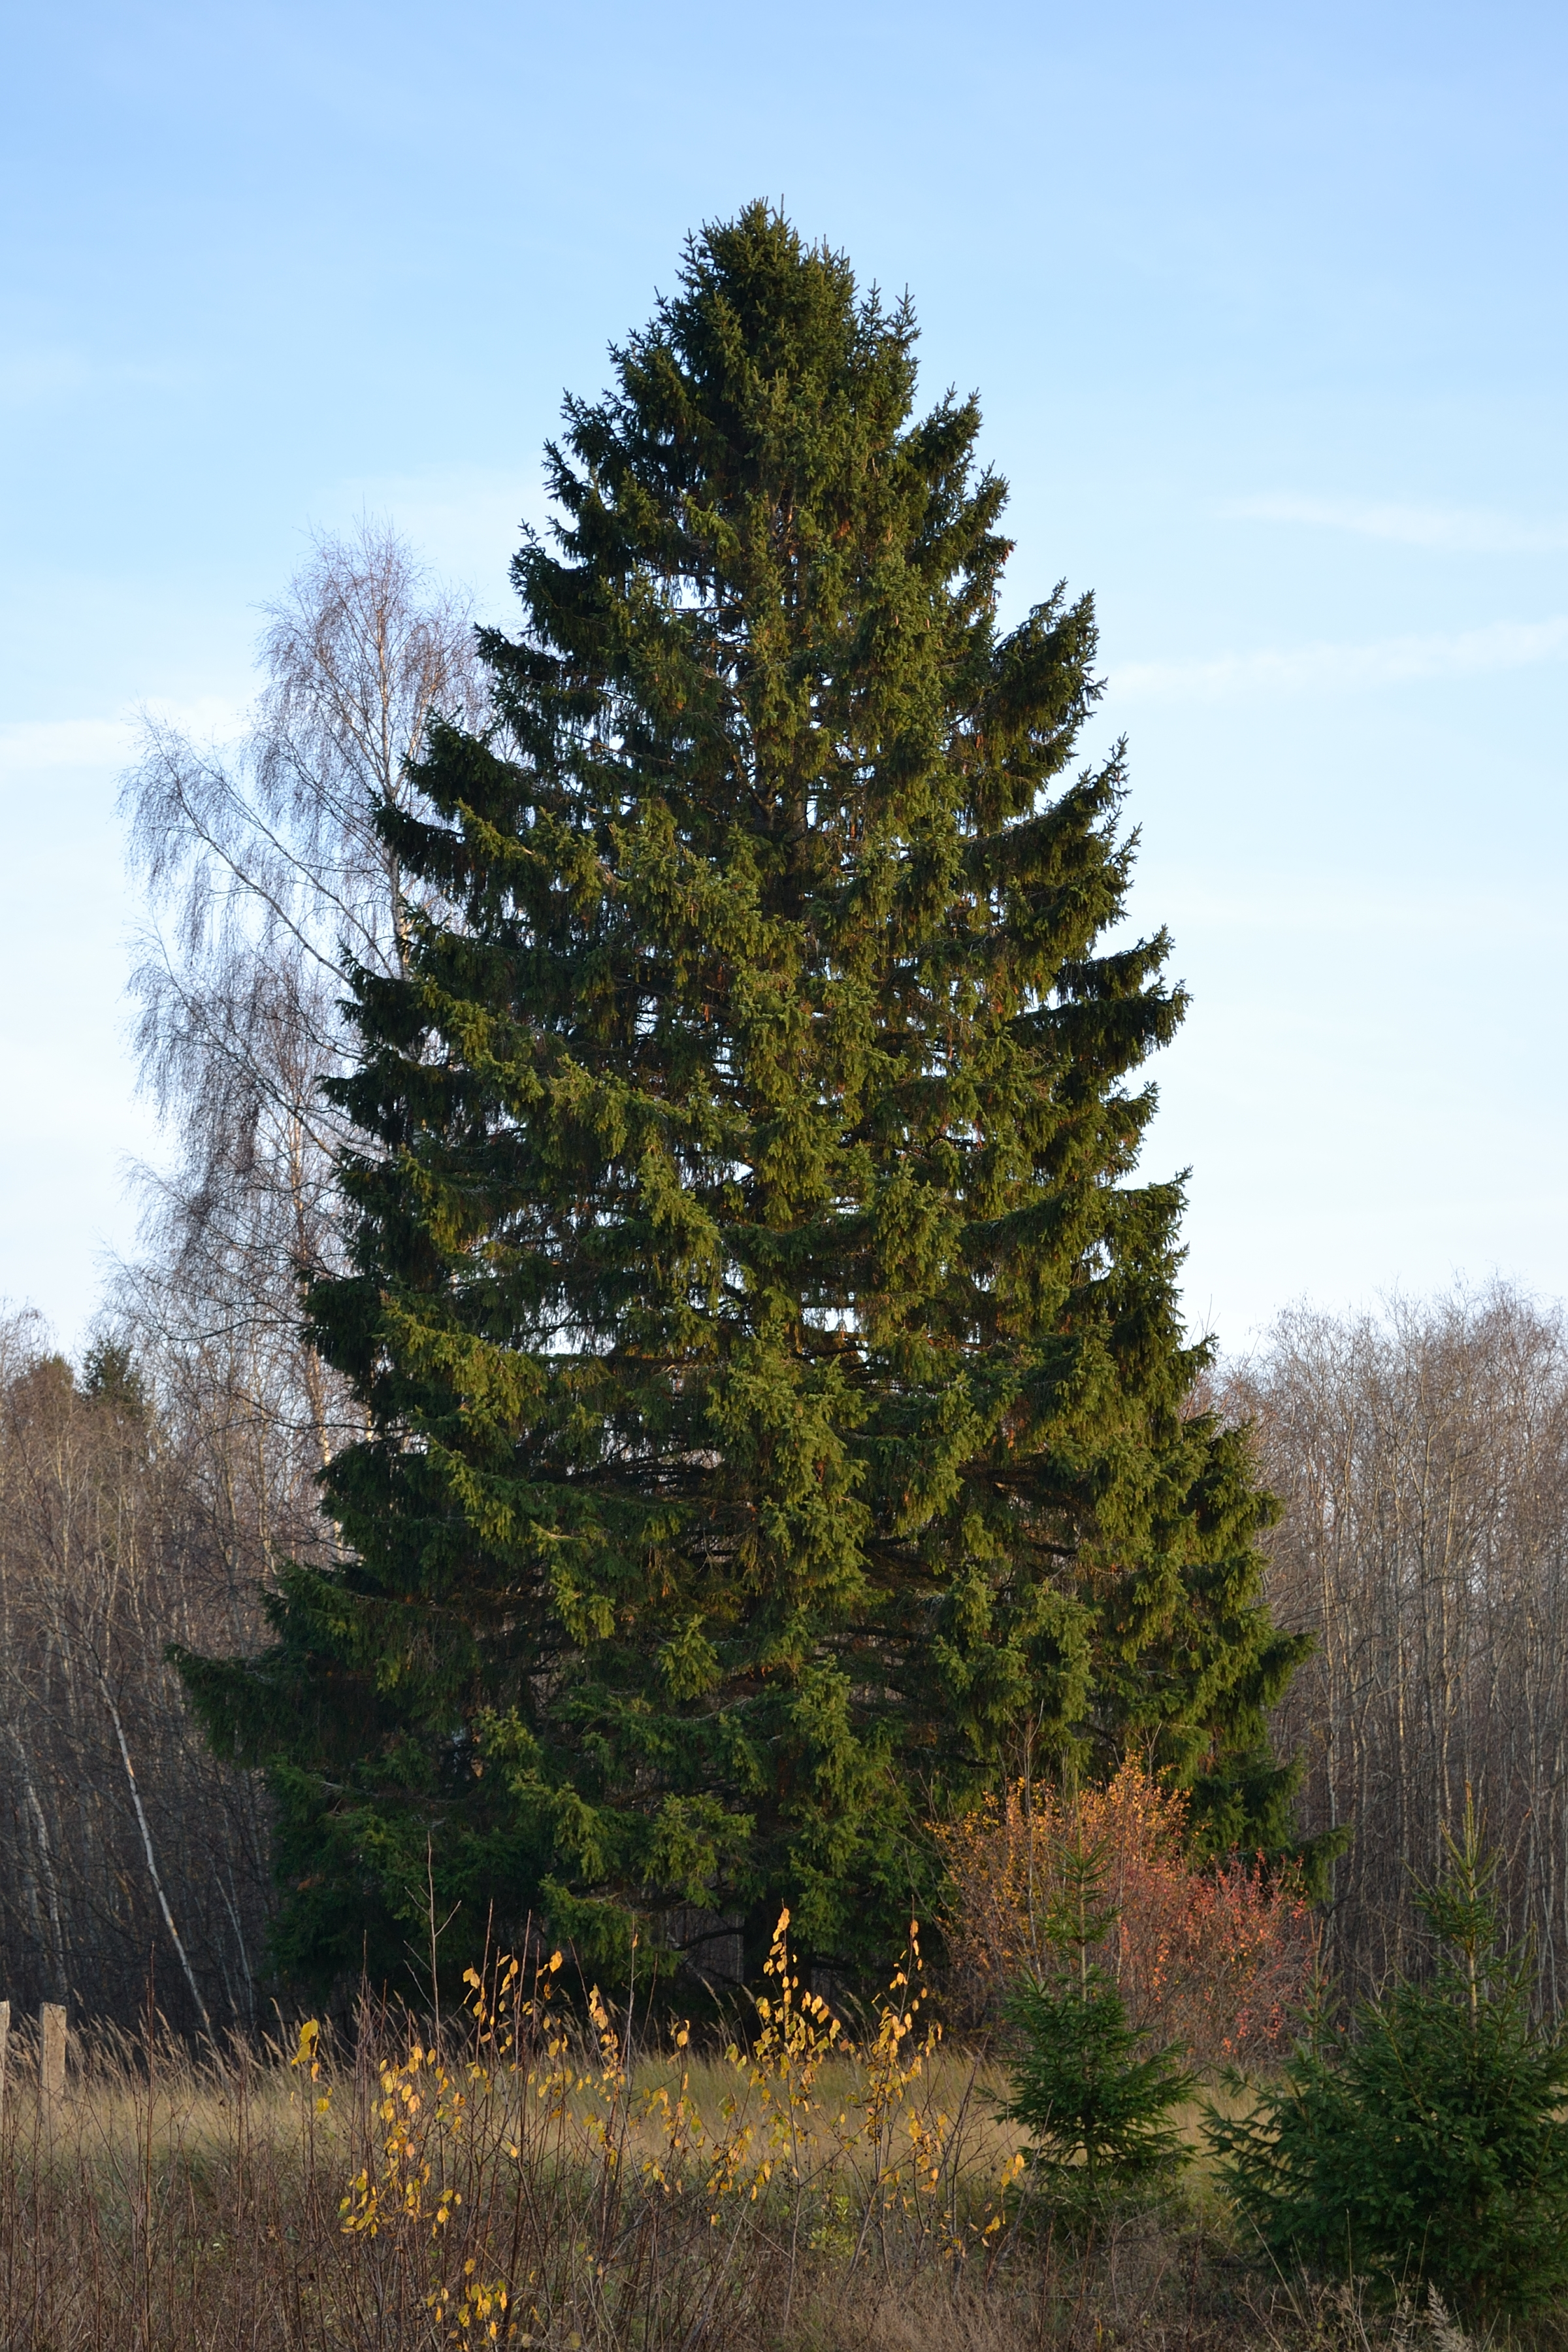
\includegraphics[width=0.8\linewidth,height=0.9\linewidth]{imaxes/picea.jpg}
    \caption{Imagen de una picea}
  \end{subfigure}
\end{figure}

Para corroborar esto se escogieron 29 de los 70 tiles anteriores donde predominan los caducifolios y donde las nube de puntos tiene una buena densidad. Esta vez los parámetros los ajustamos para este tipo de bosque y nos quedaron como vemos en la tabla \ref{tablavar2}

\begin{table}[h]
\centering
\rowcolors{2}{white}{udcgray!25}
\begin{tabular}{c|c}
\rowcolor{udcpink!25}
\textbf{Especificación} & \textbf{Valor} \\\hline


Resolución del mapa de altura & 0.005 \\
Tamaño de vecindad & 140 \\
Umbral detección en máximos & 0.3 \\
Mínimo de puntos por estrato & 40 \\
Tamaño de "Slice" & 1 \\
Umbral Linealidad & 0.1 \\

\end{tabular}
\caption{Tabla con el valor de las constantes para el test en caducifolios}
\label{tablavar2}
\end{table}

Tras ejecutar el mismo algoritmo en este dataset obtenemos los resultados que podemos ver en la tabla \ref{tablaconf2} y \ref{tablaMetr2} que podemos ver que son totalmente diferentes.

\begin{table}[!h]
\centering
\rowcolors{2}{white}{udcgray!25}
\begin{tabular}{c|c|c}
\rowcolor{udcpink!25}
\textbf{True positives} & \textbf{False Negatives} & \textbf{False Positives} \\\hline
139 & 15 & 46 \\
\end{tabular}
\caption{Valores de la matriz de confusión en el nuevo dataset}
\label{tablaconf2}
\end{table}
\begin{table}[!h]
\centering
\rowcolors{2}{white}{udcgray!25}
\begin{tabular}{c|c|c|c}
\rowcolor{udcpink!25}
\textbf{Accuracy} & \textbf{Precision} & \textbf{Recall} & \textbf{F1 Score} \\\hline
72 \% & 82 \% & 90 \% & 83 \% \\
\end{tabular}
\caption{Métricas obtenidas con los valores de la matriz en el nuevo dataset}
\label{tablaMetr2}
\end{table}

Aquí vemos como ahora no tenemos una precisión mayor y nuestro sistema es mas exacto, la precisión tiene un porcentaje de mejora del 20 \% lo que es bastante, el Recall se mantiene por la cantidad de árboles que detectamos sigue siendo alta. En general podemos ver mejores resultados este tipo de entorno, pero aun así esto podría estar condicionado por la densidad de puntos, para un análisis mas exhaustivo seria necesario tener un conjunto de datos de pruebas con varias especies y con densidades de puntos mas altas que estas, estas se podrían obtener mediante escaneos terrestres o con drones con un sensor equipado.

Por último comentar los tiempos de ejecución, la ejecución del entorno de prueba tomo 59 segundos lo que es un valor bastante alto si lo relacionamos con lo que realmente tardaríamos en procesar 2 tiles enteros.
Cada Tile lo dividimos en 320 subtiles aproximadamente, es decir los dos tiles serian 740 subtiles. Si hacemos una regla de tres con los 59 segundos que tarda en ejecutar 70 tiles tendríamos que tardaría 10 minutos en procesar los 2 tiles. En el capitulo \ref{chap:conclusions} comentaremos opciones para mejorar este resultado.


\begin{figure}[h]
\centering
  \begin{subfigure}{0.5\textwidth}
    \centering
    \includegraphics[width=0.9\linewidth]{imaxes/detectcad1.png}
    \caption{Árboles detectados vista superior}
    \label{fig:last1}
  \end{subfigure}%
  
  \begin{subfigure}{0.45\textwidth}
    \centering
    \includegraphics[width=0.9\linewidth]{imaxes/detecad1lat.png}
    \caption{Árboles detectados vista lateral}
    \label{fig:last2}
  \end{subfigure}%
  
  \begin{subfigure}{0.45\textwidth}
    \centering
    \includegraphics[width=0.9\linewidth]{imaxes/grountCad.png}
    \caption{Ground Truth}
    \label{fig:last3}
  \end{subfigure}
  
  \caption{Ejemplo de Detección en Caducifolios}
  \label{fig:algo2}
\end{figure}


\begin{figure}
  \begin{subfigure}{0.5\textwidth}
    \centering
    \includegraphics[width=0.8\linewidth,height=0.9\linewidth]{imaxes/centroidesCad1.png}
    \label{fig:last1}
  \end{subfigure}%
  \begin{subfigure}{0.5\textwidth}
    \centering
    \includegraphics[width=0.8\linewidth,height=0.9\linewidth]{imaxes/centroidesCad2.png}
    \label{fig:last}
  \end{subfigure}
 \caption{Ejemplo de los centroides que forman una linea para caducifolios}
  \label{fig:algo2}
\end{figure}